Based on the presented idea, we design and present the prototype which consists of three components (see Figure \ref{fig:figure1}):
\begin{itemize}
\item The server centrally manages all users information, bookings and machines status.
\item Each washing machine has a monitoring device which displays current states of the machine and communicate with server.
\item {\toolname} is the laundry booking application on mobile phone.
\end{itemize}
\begin{figure}[h]
\centering
  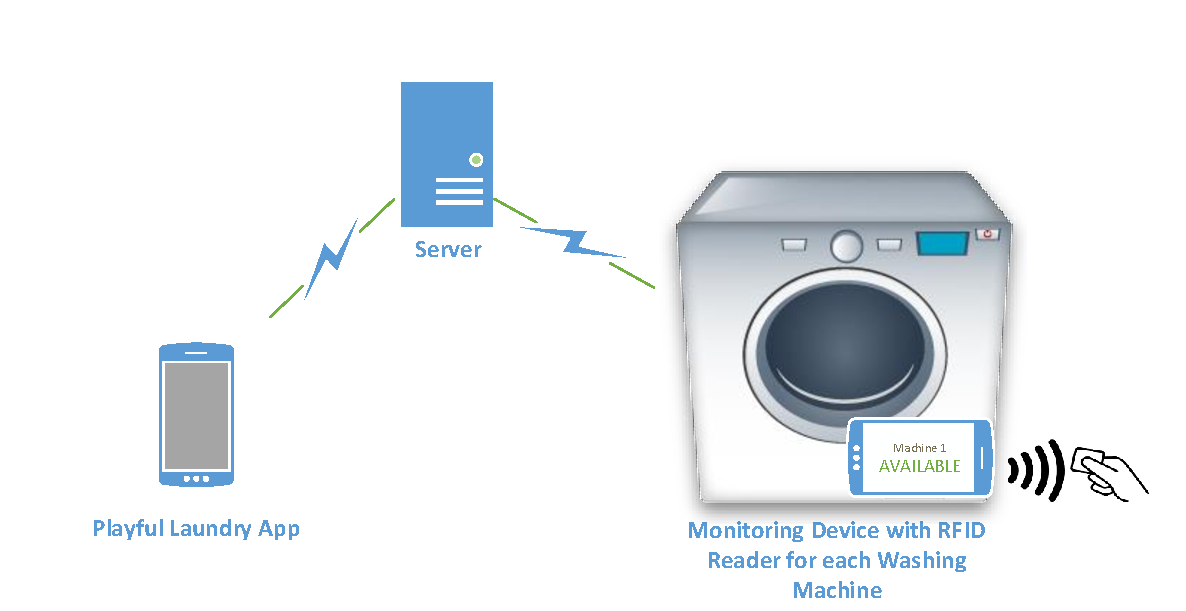
\includegraphics[width=\columnwidth]{figures/overview}
  \caption{Three components of the booking system.}~\label{fig:figure1}
\end{figure}
\subsubsection{Monitoring Device}
Each monitoring device has a RFID reader and a screen which displays interactive instruction and information of the machine such as: machine id, remaining time of current job, current state of washing machine (\emph{AVAILABE} - there is still enough time before the next reservation begins, \emph{USED IN A MOMENT} - next reservation will begin shortly, \emph{RESERVED} - the machine was already booked at that moment, \emph{IN USE} - machine is running, \emph{FINISHED} - washing has just finished), etc.
 For prototyping monitoring device, we use an android phone as a display and an arduino uno board with RFID shield (see Figure \ref{fig:figure2}).
\begin{figure}[h]
\centering
  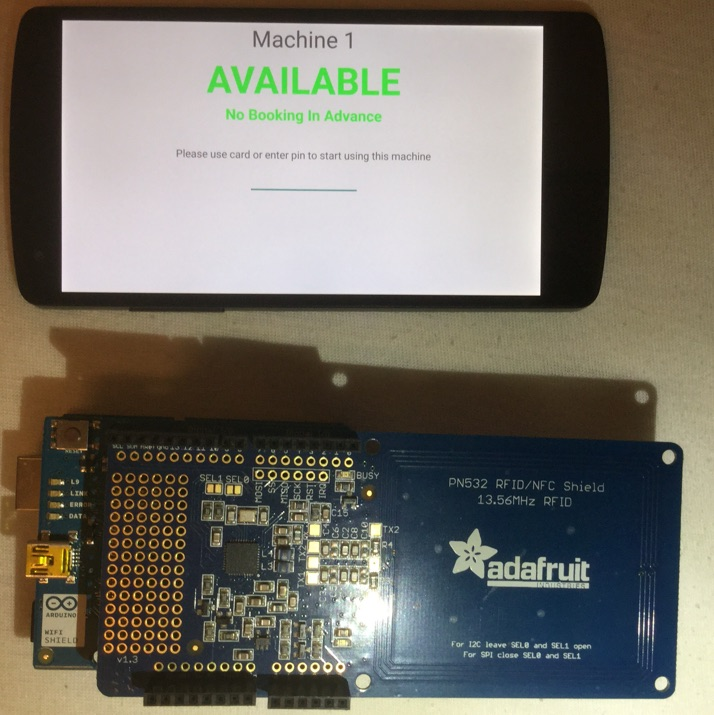
\includegraphics[width=0.7\columnwidth]{figures/Monitoring}
  \caption{The prototype of monitoring device.}~\label{fig:figure2}
\end{figure}
To activate a machine, users could either scan their RFID cards or enter PIN number. If the users already reserved the current time slot, monitoring device would instruct them to start the machine; otherwise they have go through booking process right on the monitoring device before using the machine.

When the machine is \emph{IN USE} or \emph{FINISHED} state, the \emph{booking id} of current session would be showed on the screen. Figure \ref{fig:figure3} shows the screenshot of the display when the machine is \emph{IN USE}. This id disappears once the users take their clothes out of the machine. Therefore, if the users are being late, other users could use this \emph{booking id} and the \emph{machine id} for reporting.
\begin{figure}[h]
\centering
  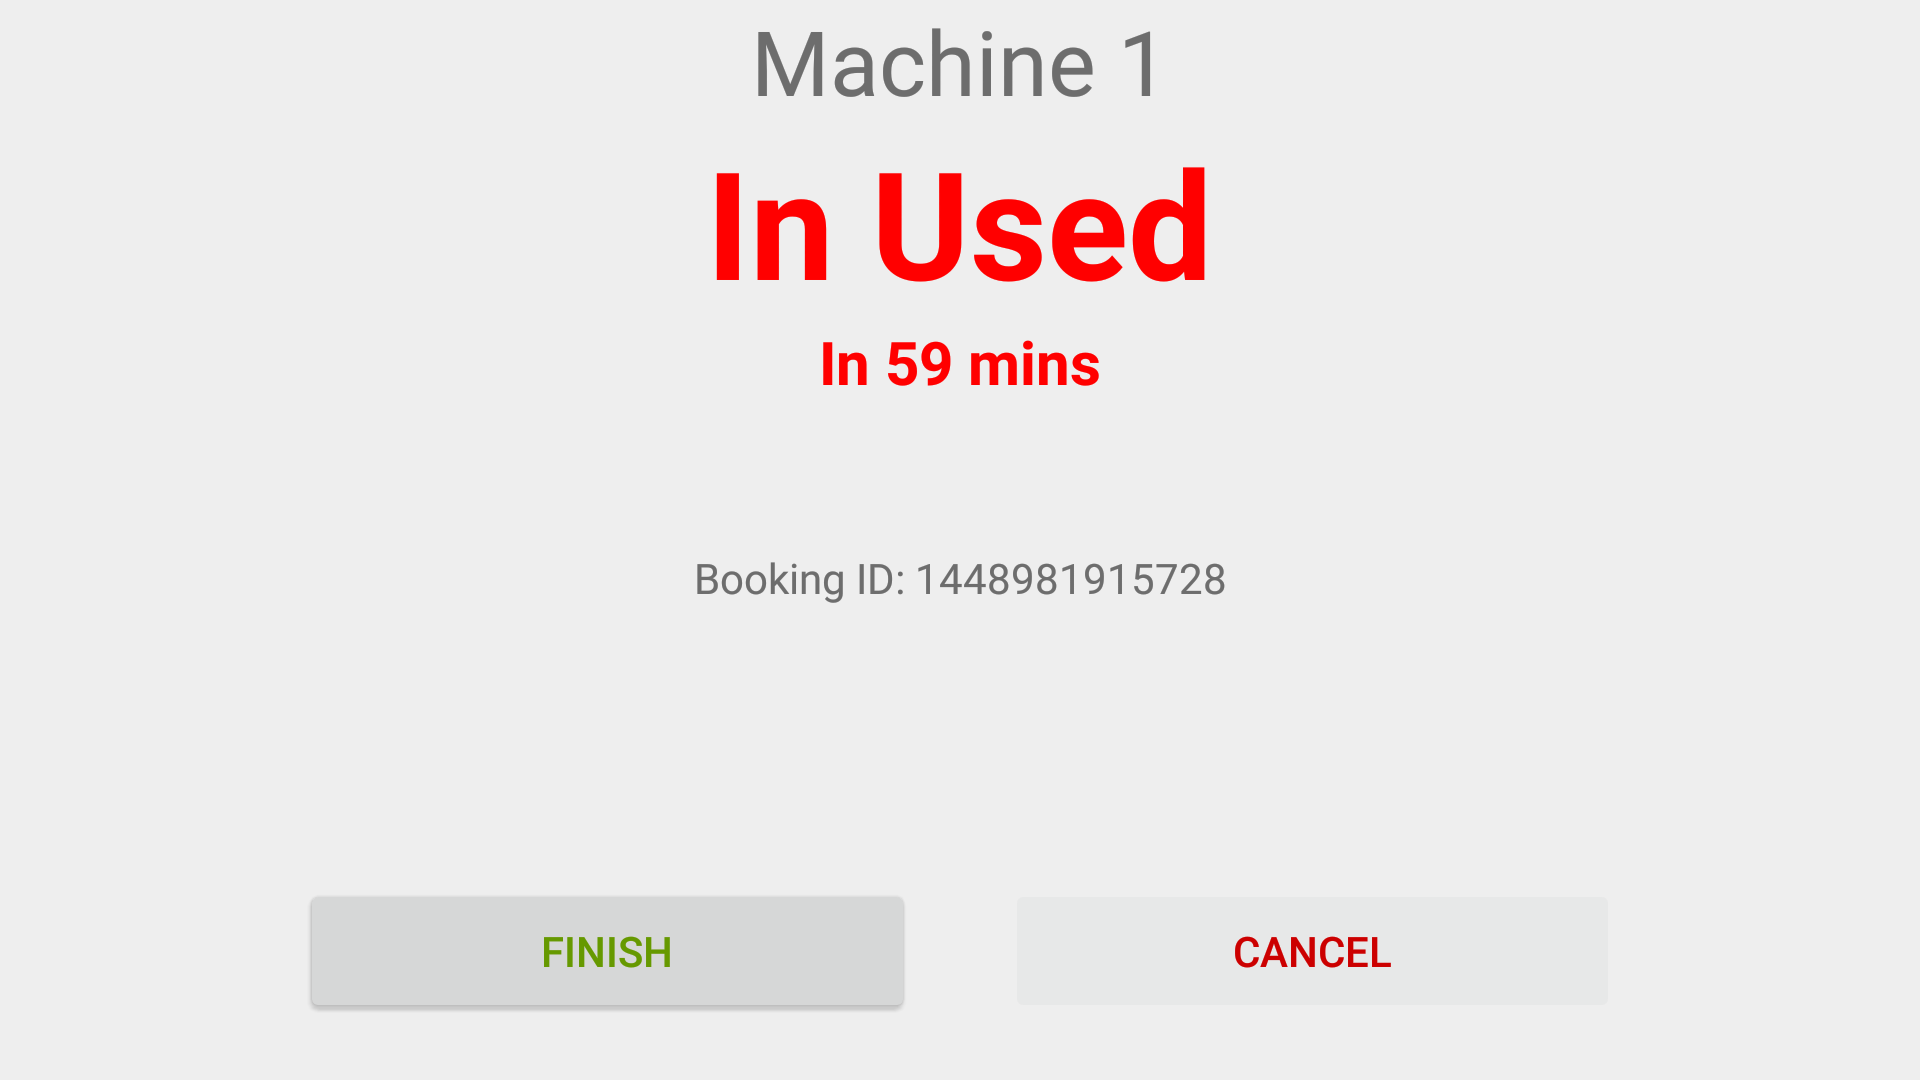
\includegraphics[width=0.8\columnwidth]{figures/inuse}
  \caption{Monitoring display when the machine is running.}~\label{fig:figure3}
\end{figure}
\subsubsection{{\toolname} Application}
{\toolname} is an android application which allows users to reserve a washing machine, manage booking, observe the current states of the machines, etc. Figure \ref{fig:menu} shows the menu of the application.

\begin{figure*}%
    \centering
    \subfloat[Main menu]{{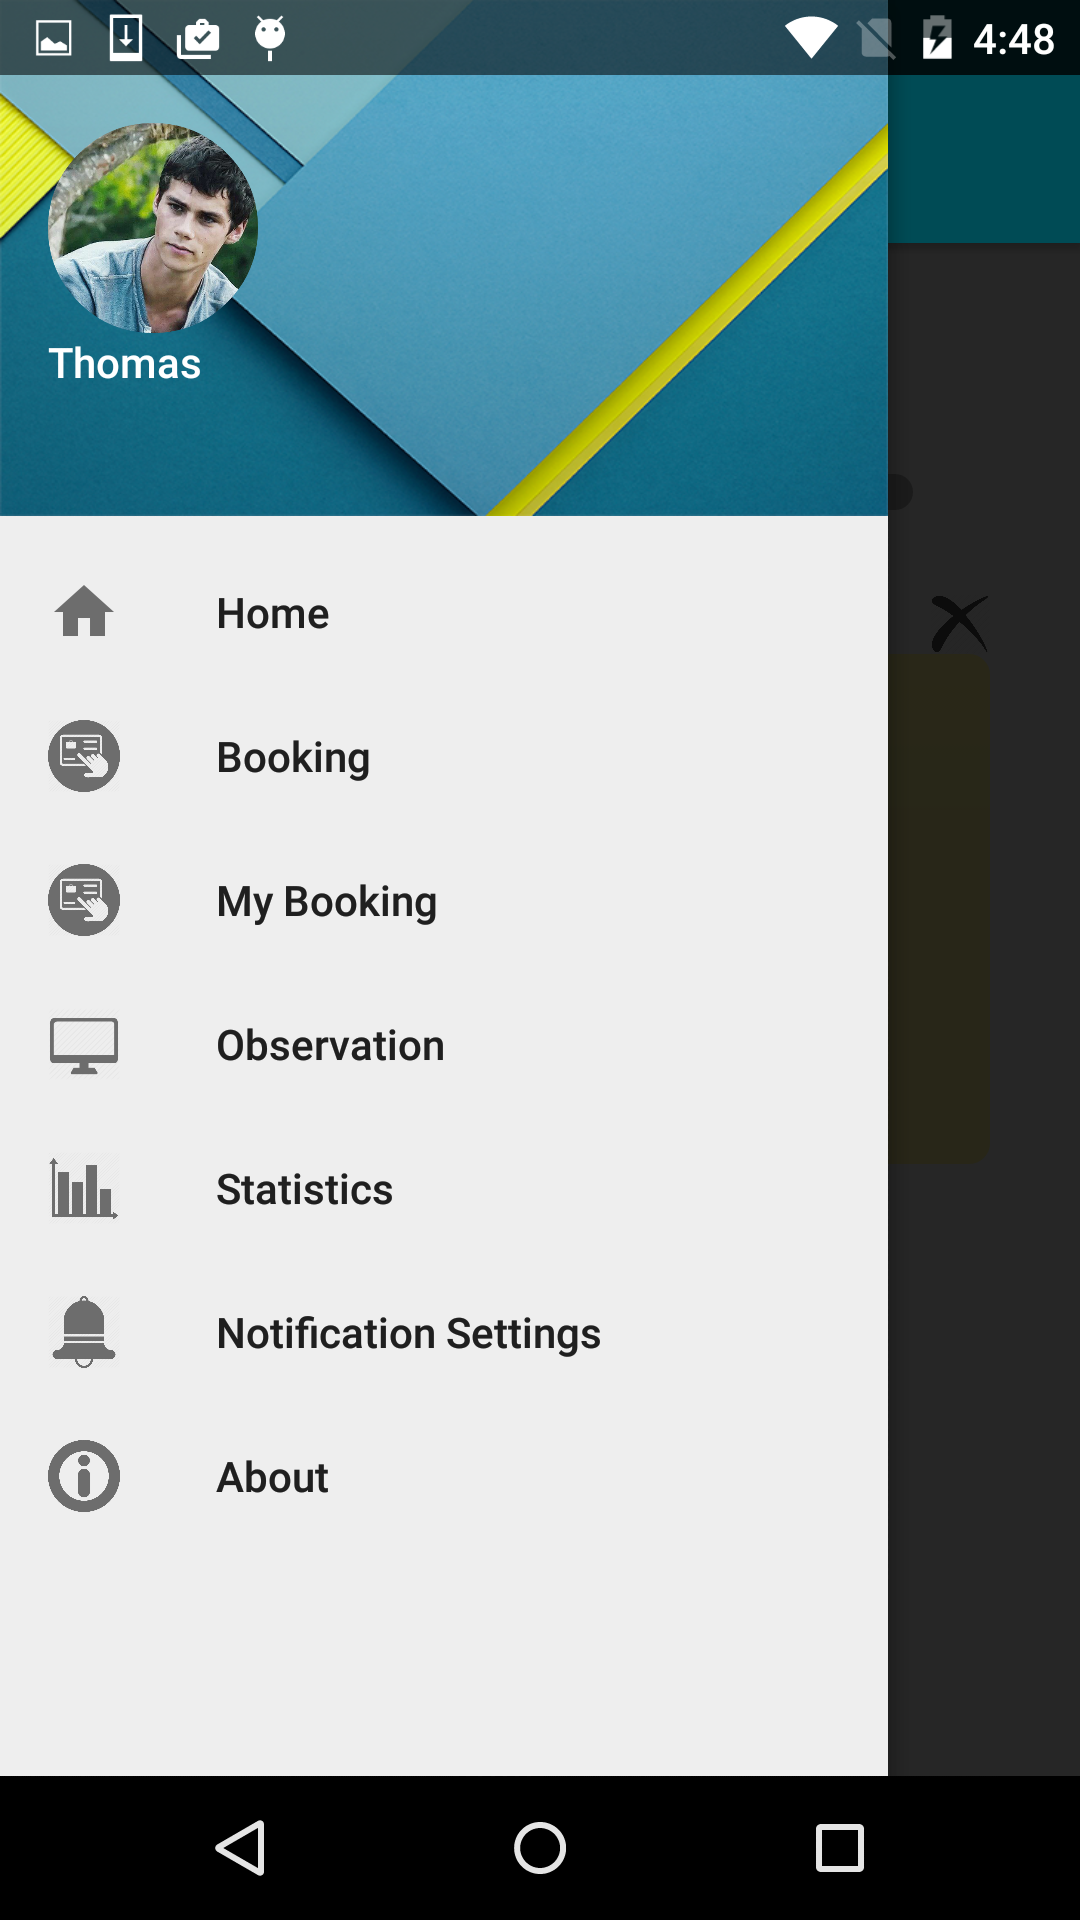
\includegraphics[width=0.4\columnwidth]{figures/menu} \label{fig:menu}}}
    %\qquad
    \subfloat[Home]{{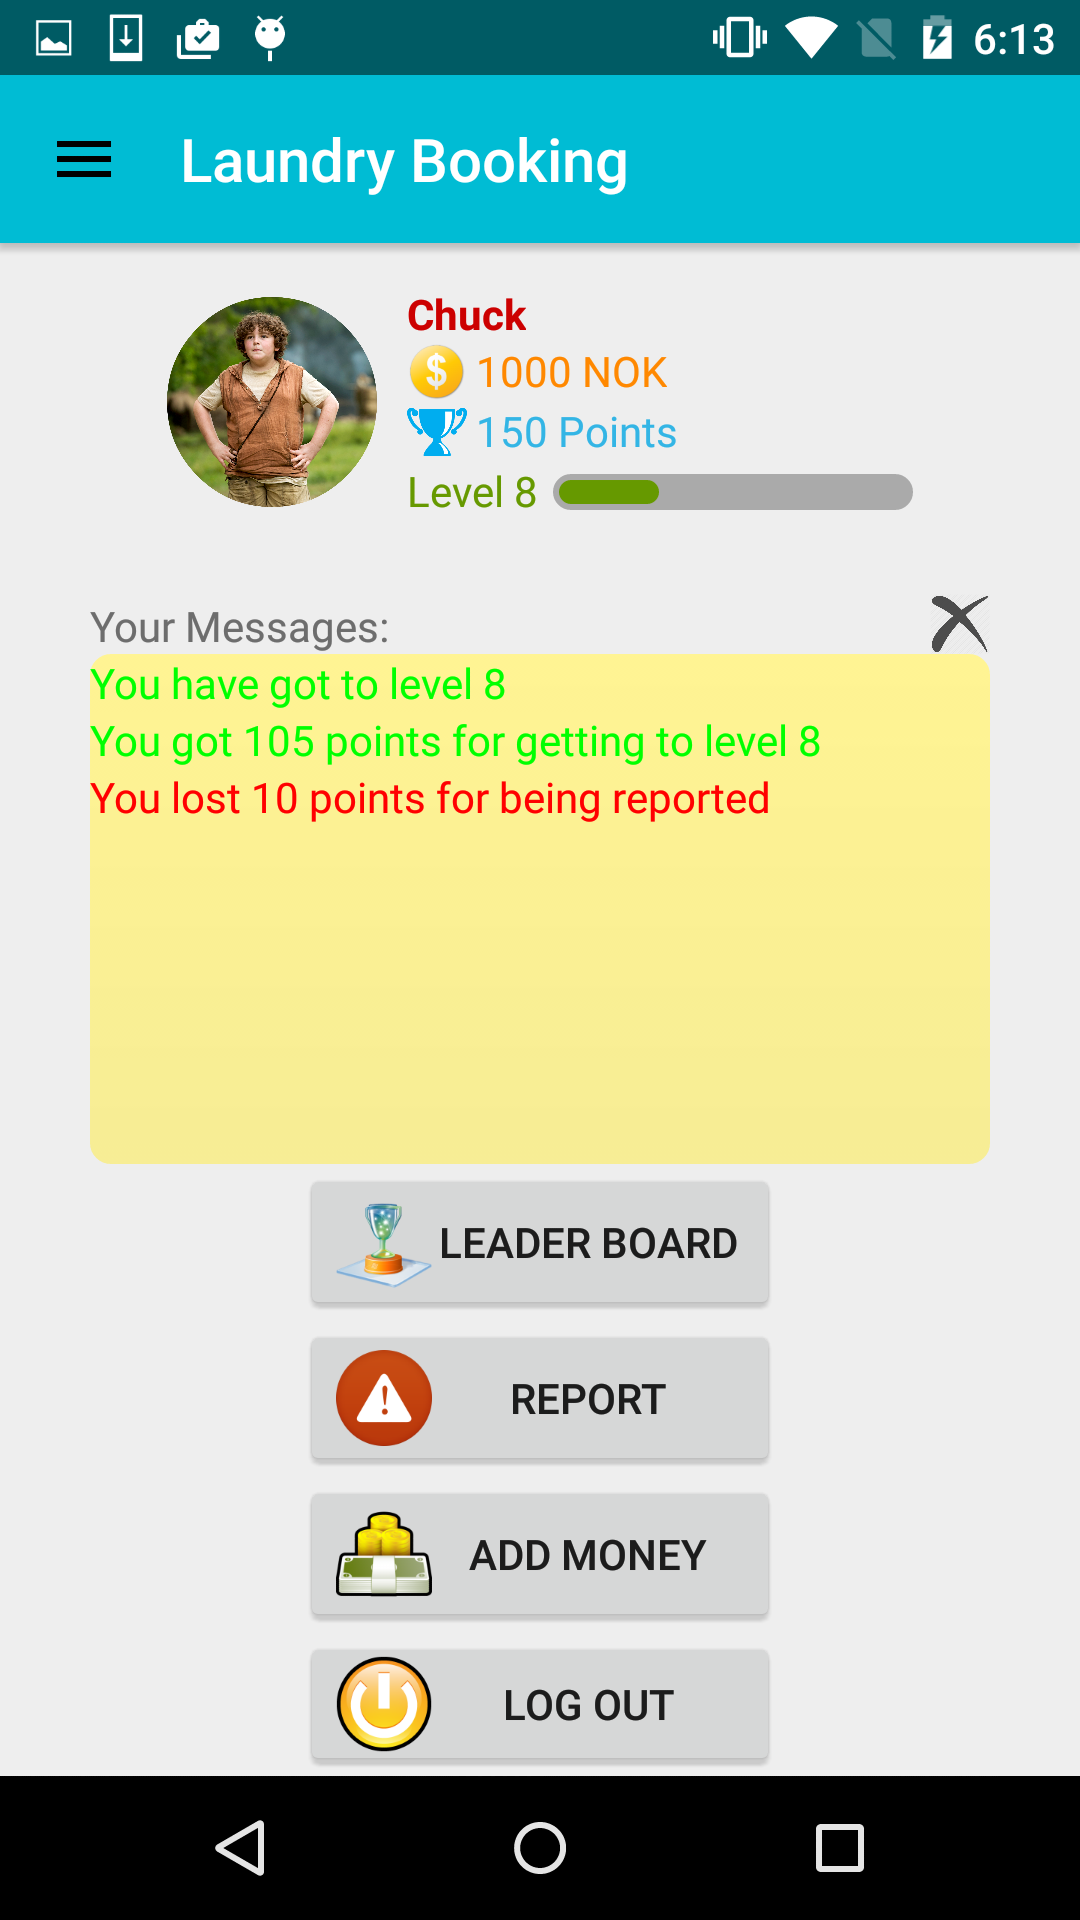
\includegraphics[width=0.4\columnwidth]{figures/home} \label{fig:home} }}
		\subfloat[Booking]{{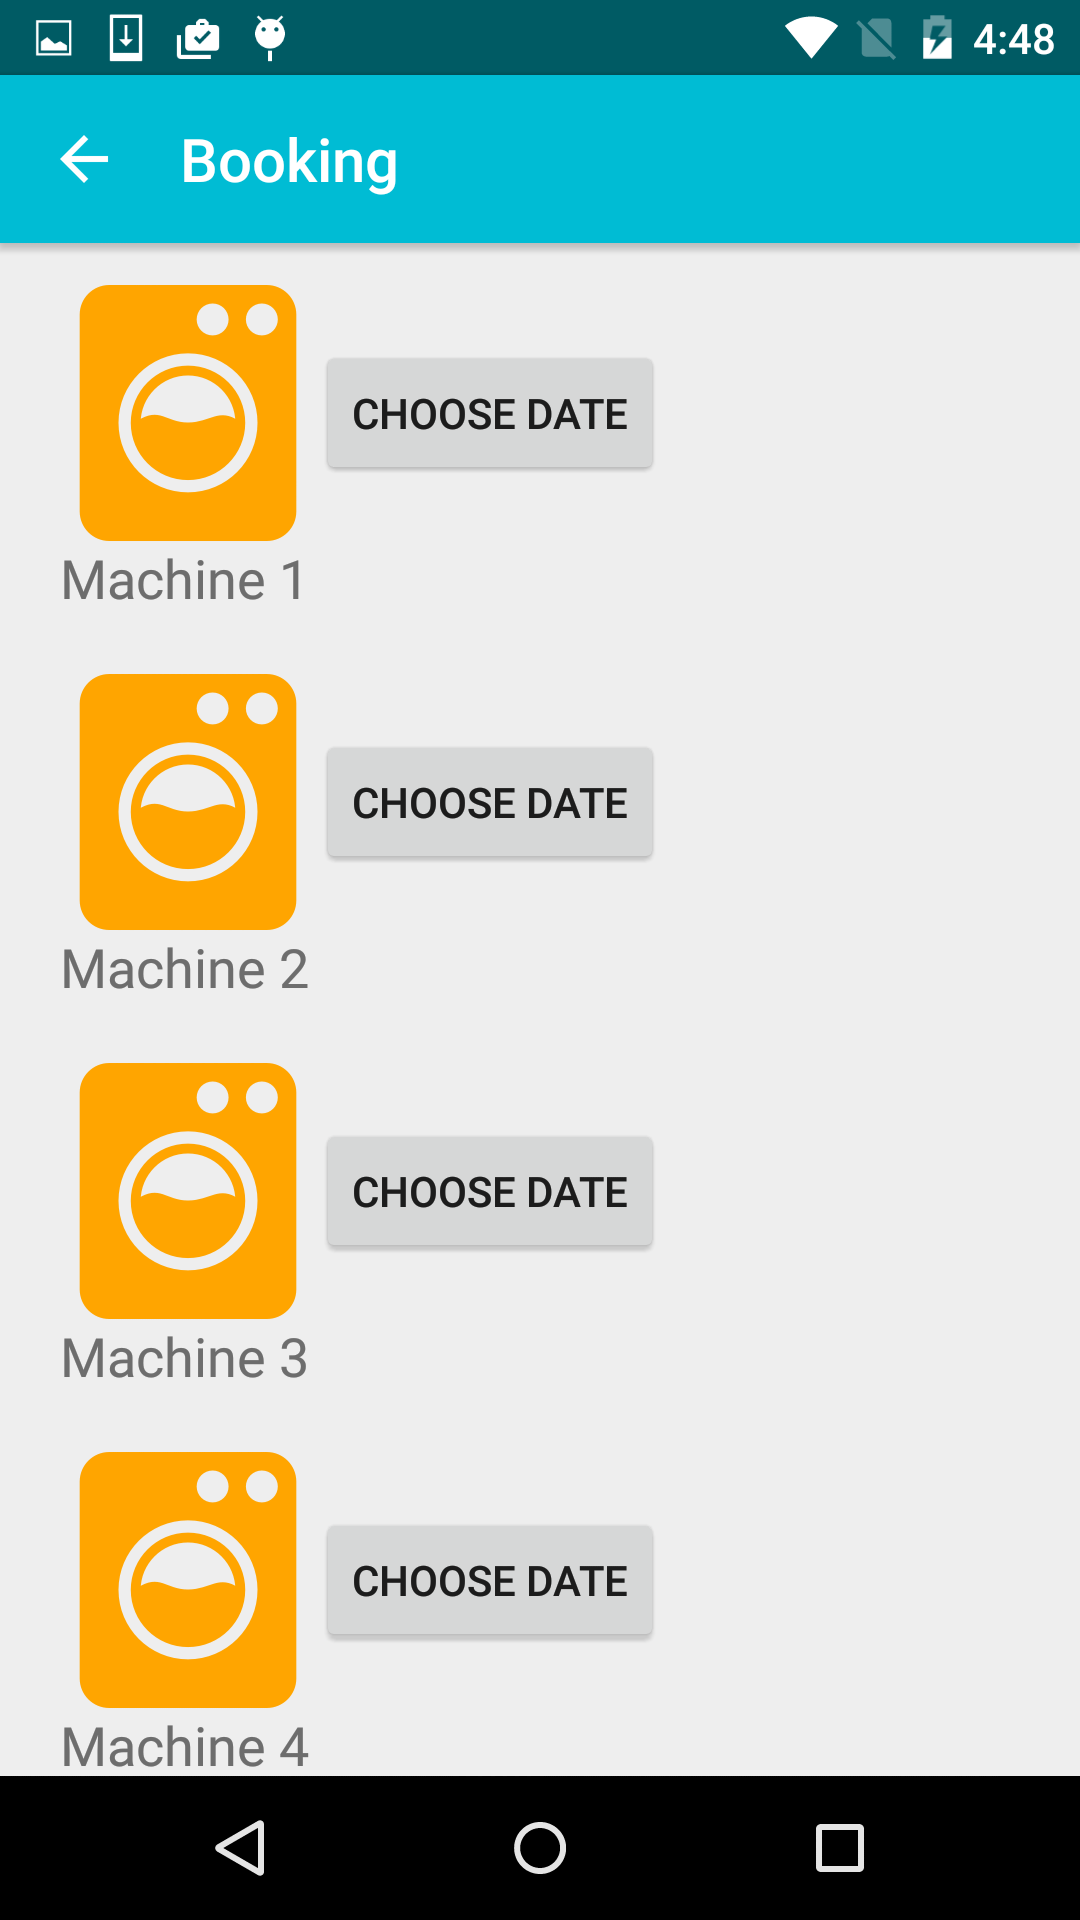
\includegraphics[width=0.4\columnwidth]{figures/booking} \label{fig:booking} }}
		\subfloat[Observation]{{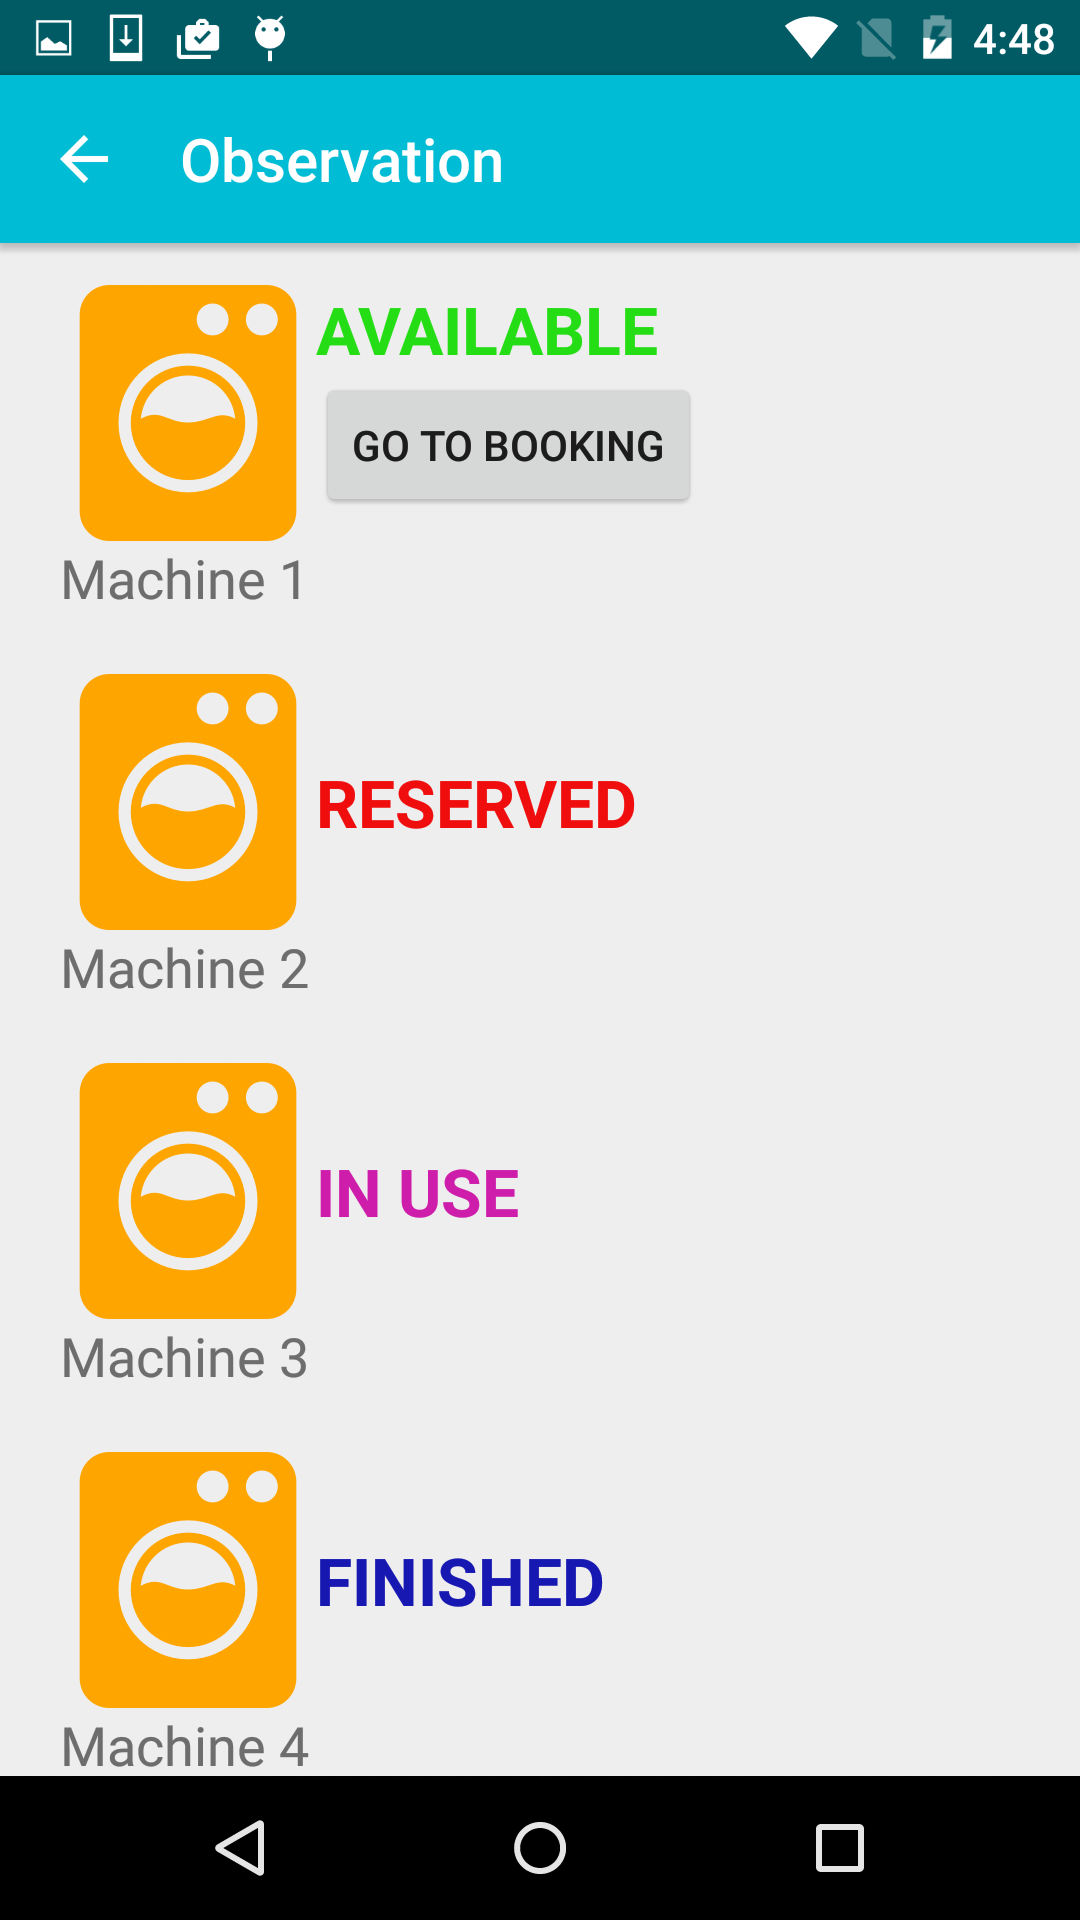
\includegraphics[width=0.4\columnwidth]{figures/observation} \label{fig:observation} }}
		\subfloat[Statistics]{{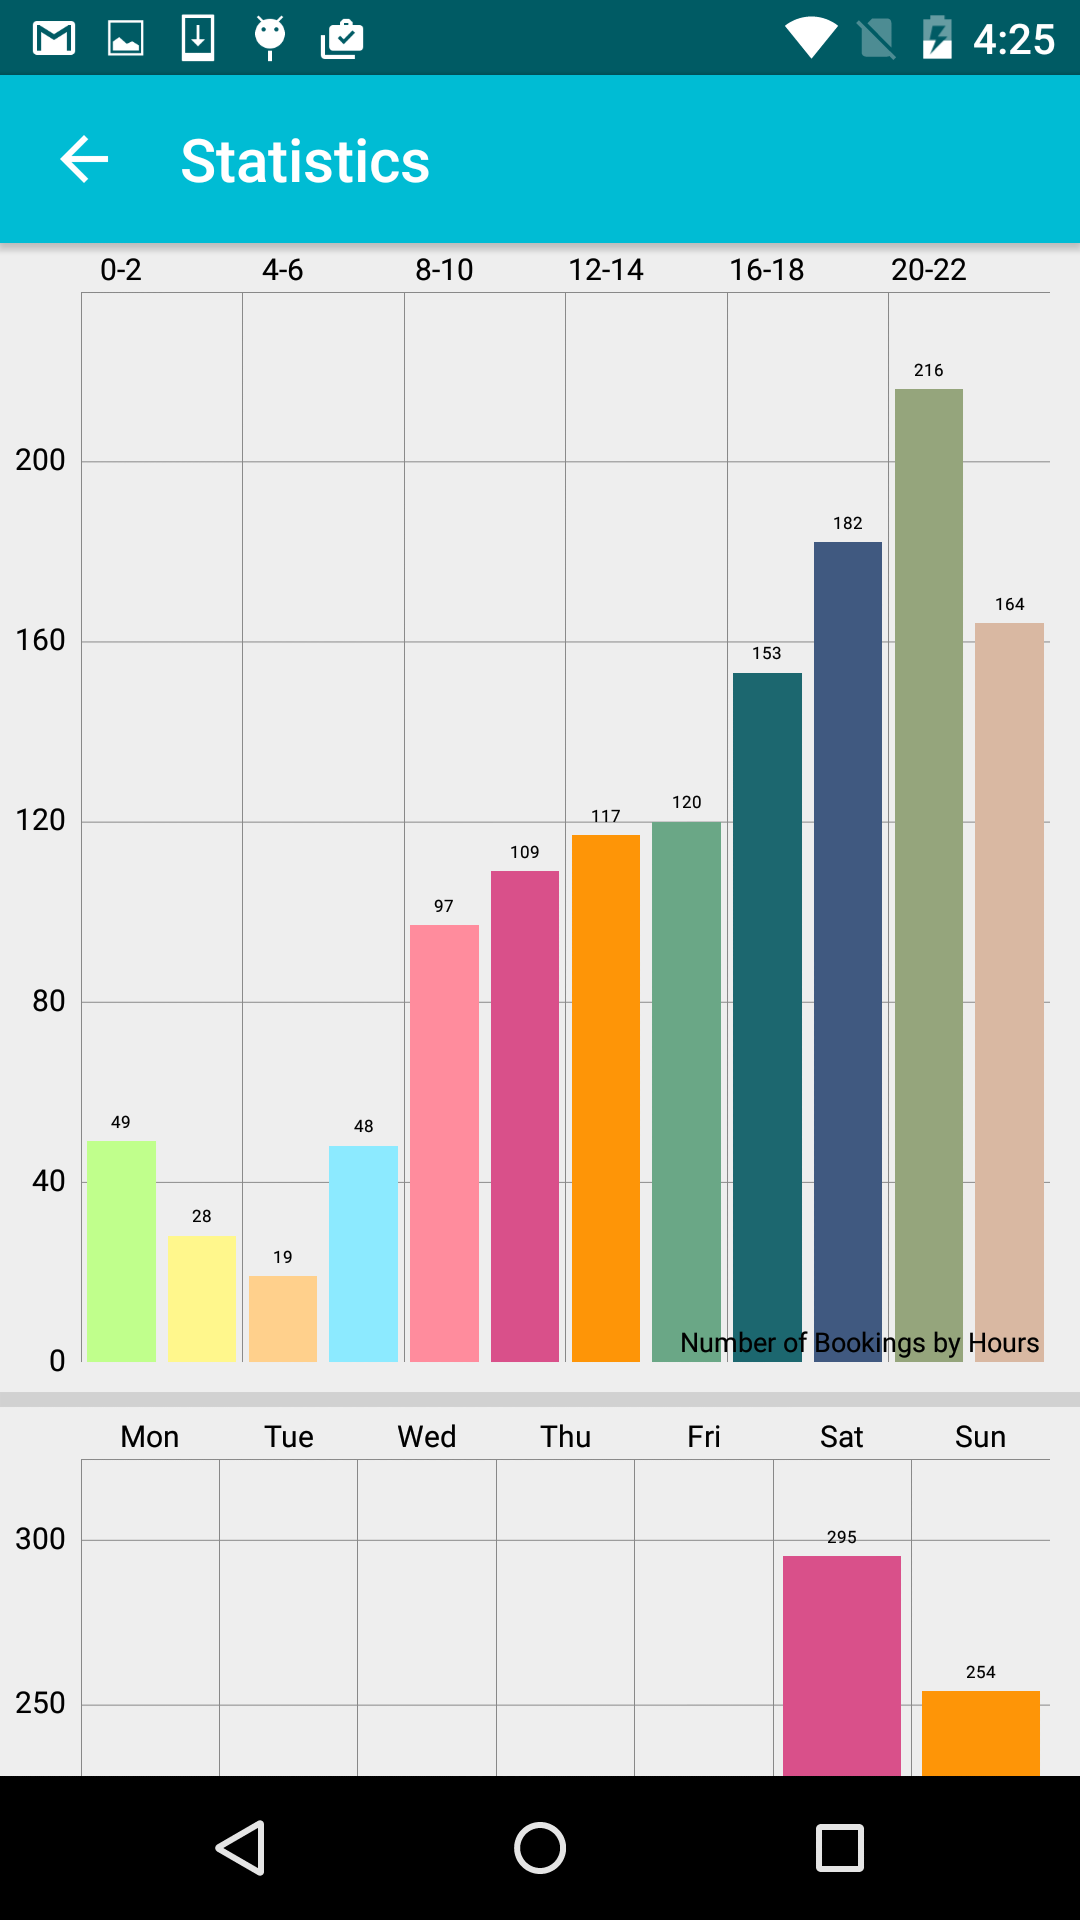
\includegraphics[width=0.4\columnwidth]{figures/stat} \label{fig:stat} }}
    \caption{User interface of \toolname.}%
    \label{fig:figure4}
\end{figure*}


\begin{figure}%
    \centering
    \subfloat[Time slots and award points]{{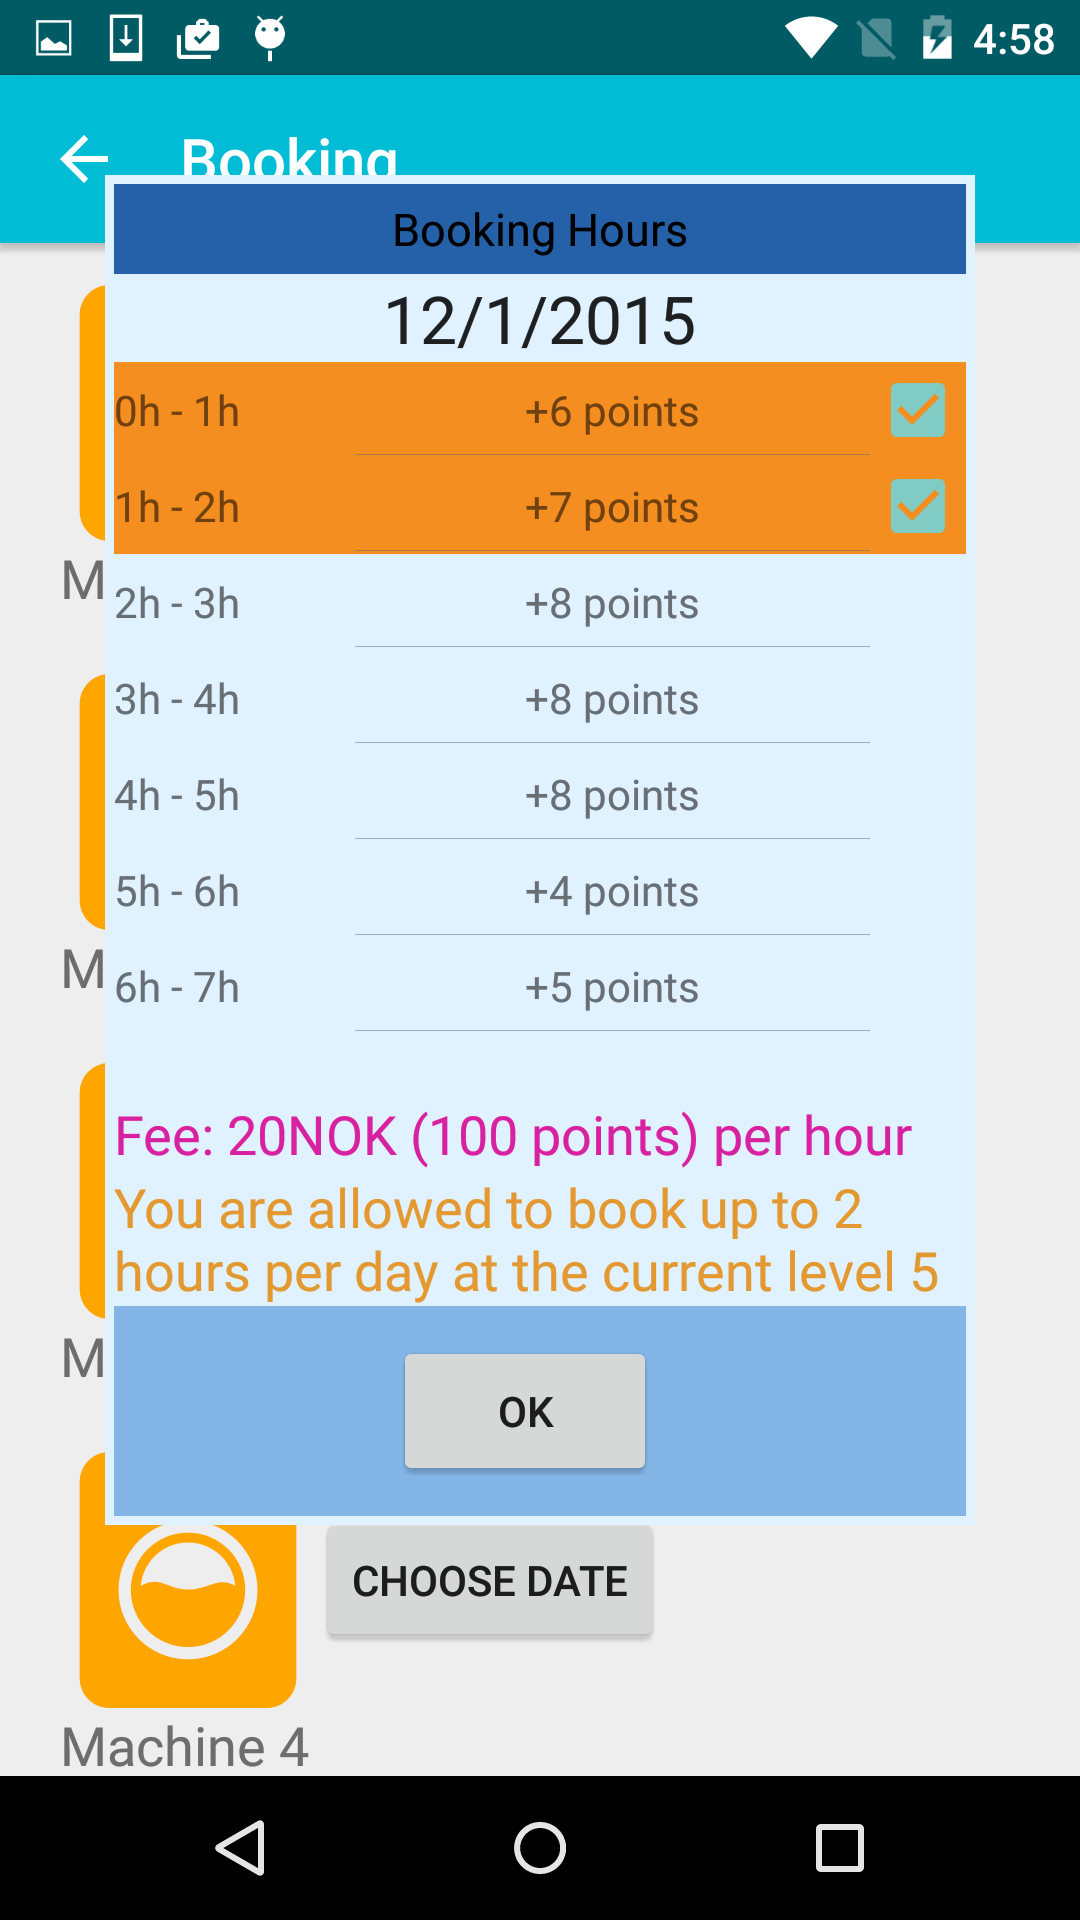
\includegraphics[width=0.4\columnwidth]{figures/hours} \label{fig:hours}}}
    %\qquad
    \subfloat[Leader Board]{{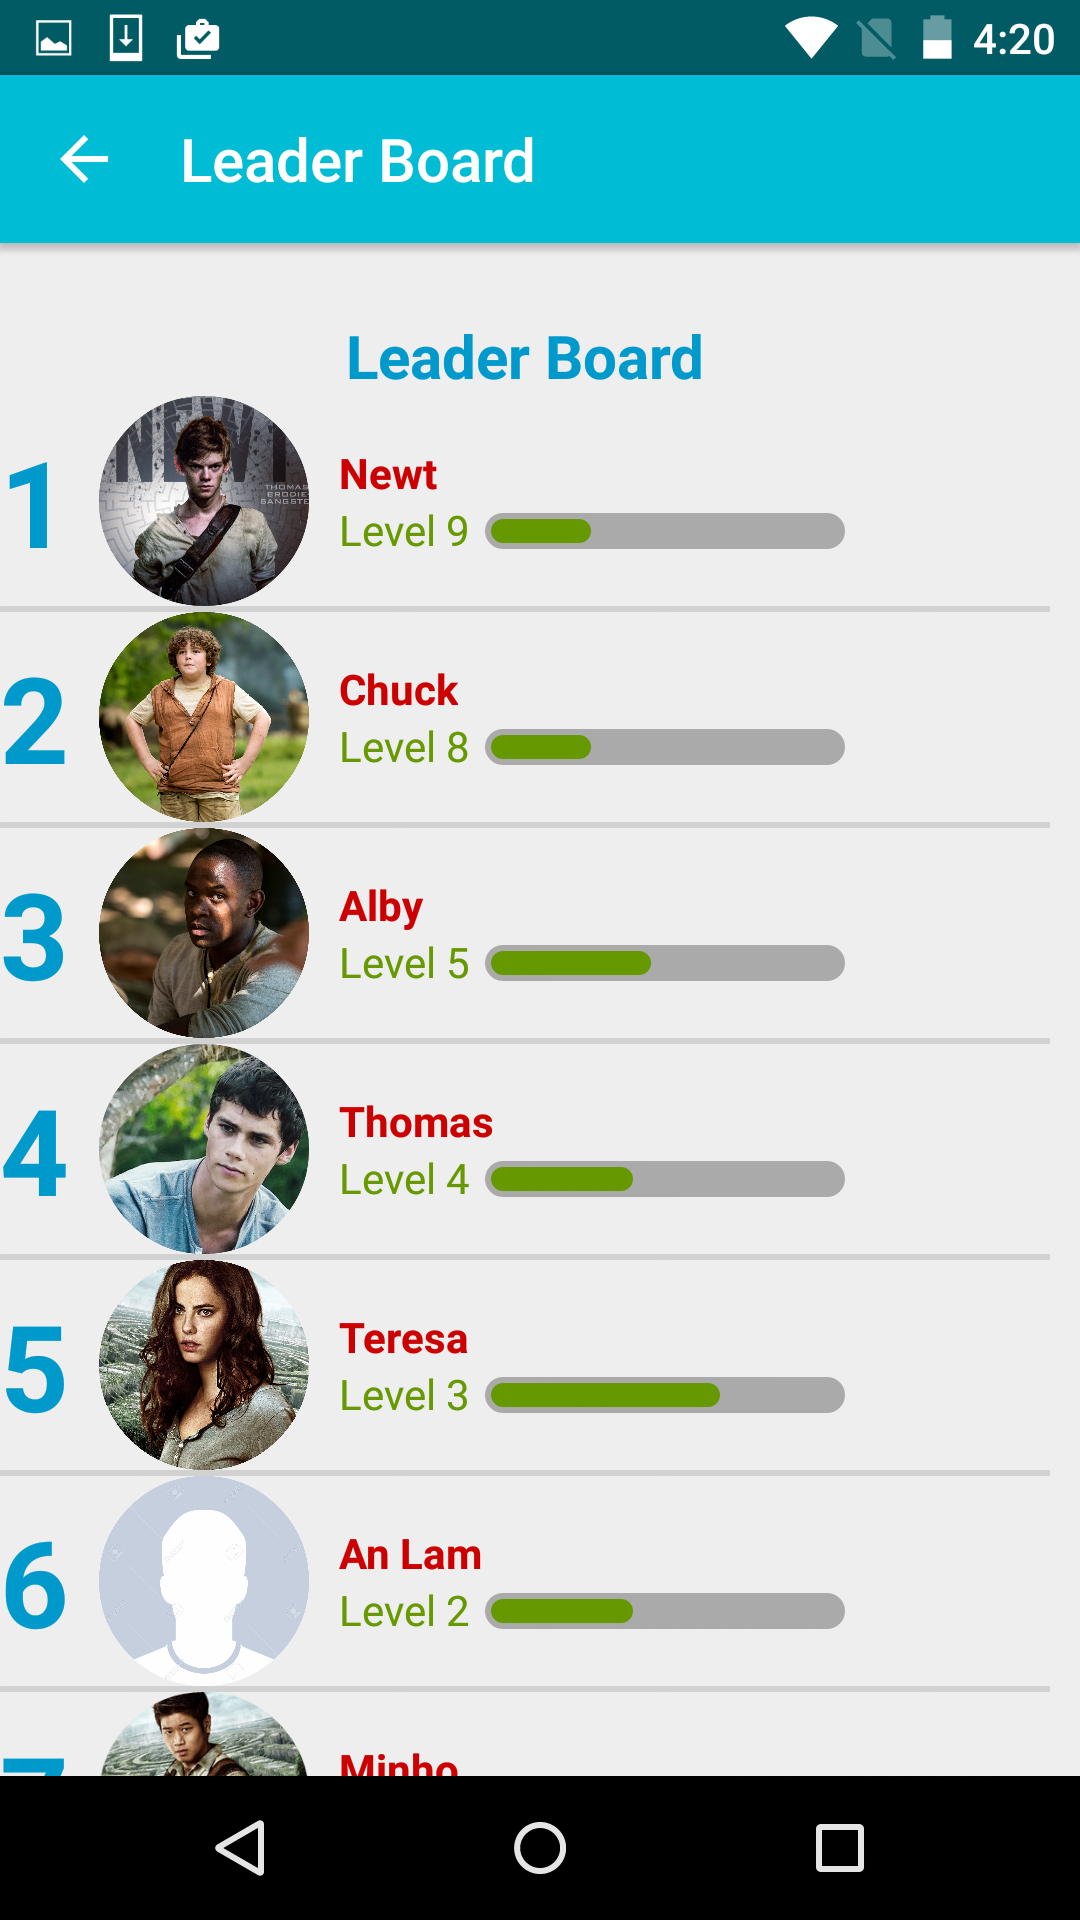
\includegraphics[width=0.4\columnwidth]{figures/leaderboard} \label{fig:leaderboard} }}
		\caption{Time slots and Leader board.}%
    \label{fig:figure5}
\end{figure}